\subsection{Interface}
\label{sect:maw_interface}

\begin{figure}
    \center{
        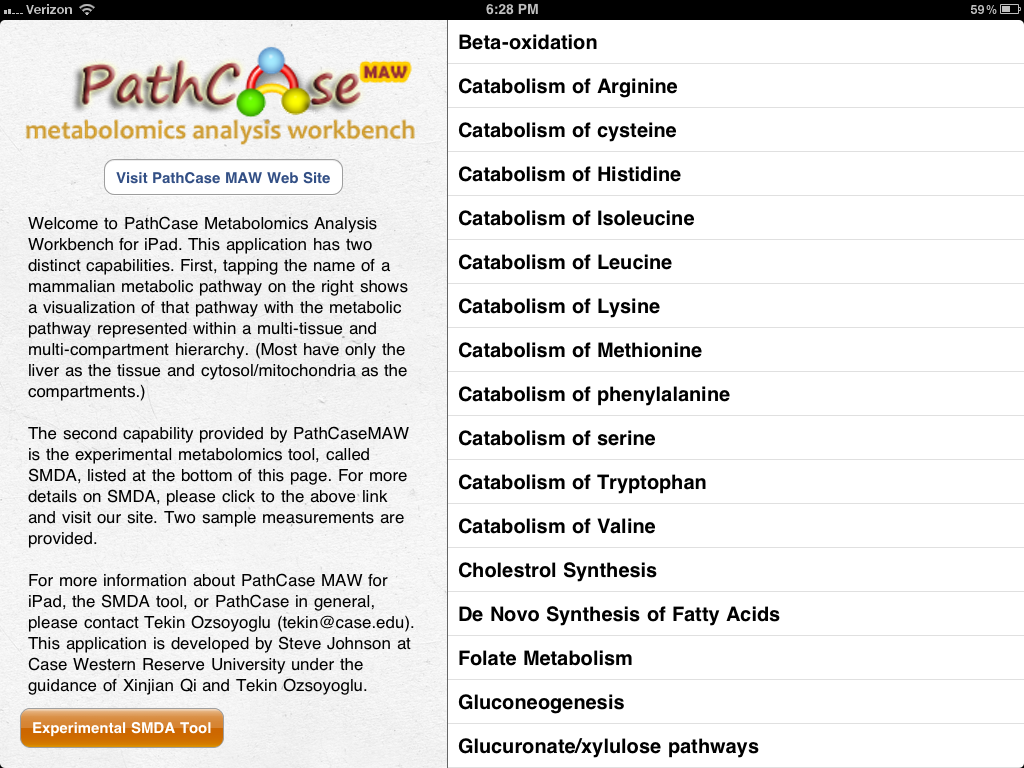
\includegraphics[width=\columnwidth]{maw/figures/screenshot_list}}
    \caption{\label{fig:maw_screenshot_list} List of pathways on the main screen
    of PathCase MAW for iPad}
\end{figure}

\begin{figure}[hbt]
    \center{
        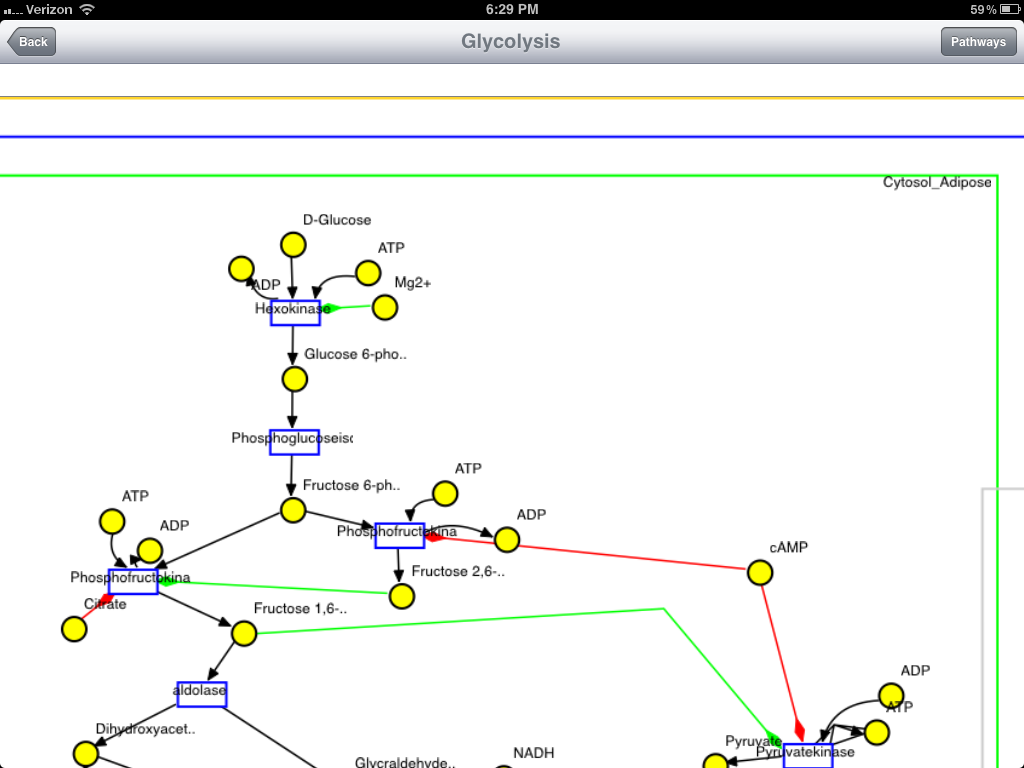
\includegraphics[width=\columnwidth]{maw/figures/screenshot_glycolysis}}
    \caption{\label{fig:maw_screenshot_pathway} Scrolling, zooming view of
    Glycolysis}
\end{figure}

The home screen of the MAW app displays a list of pathways that the user can
choose from to view a graph. This screen is shown in figure
\ref{fig:maw_screenshot_list}. It also contains a brief explanation of the
PathCase database and instructions for using the app.

After selecting a pathway, the user enters the graph view, where they can pan
and zoom across a pathway. The view for glycolysis is shown in figure
\ref{fig:maw_screenshot_pathway}.
